%% The first command in your LaTeX source must be the \documentclass command.
%%
%% Options:
%% twocolumn : Two column layout.
%% hf: enable header and footer.
\documentclass[
% twocolumn,
 hf]{ceurart}

%%
%% One can fix some overfulls
\sloppy

%\usepackage{ulem}

%%
%% Minted listings support 
%% Need pygment <http://pygments.org/> <http://pypi.python.org/pypi/Pygments>
\usepackage{listings}
%% auto break lines
\lstset{breaklines=true}
\usepackage{tikz}
\usetikzlibrary{positioning}
\definecolor{pantone_174_6}  {cmyk} {0.56,0.42,0.32,0.00}
\definecolor{pantone_117_8}  {cmyk} {1.00,0.00,0.00,0.48} % Headings
\definecolor{pantone_127_4}  {cmyk} {0.53,0.00,0.28,0.00}
\definecolor{pantone_157_8}  {cmyk} {0.48,0.00,1.00,0.00}
\definecolor{pantone_126_8}  {cmyk} {1.00,0.00,0.41,0.48}
\definecolor{pantone_151_8}  {cmyk} {0.71,0.00,1.00,0.00}
\definecolor{pantone_119_1}  {cmyk} {0.25,0.00,0.04,0.06}

%% Secondary:
\definecolor{pantone_10_7}   {cmyk} {0.00,0.23,0.86,0.00}
\definecolor{pantone_120_2}  {cmyk} {0.38,0.00,0.06,0.18}
\definecolor{pantone_24_8}   {cmyk} {0.00,0.57,0.00,0.00}
\definecolor{pantone_149_4}  {cmyk} {0.50,0.00,0.63,0.15}
\definecolor{pantone_46_8}   {cmyk} {0.00,0.91,0.92,0.22}
\definecolor{pantone_124_16} {cmyk} {1.00,0.00,0.41,0.13}
\definecolor{pantone_74_7}   {cmyk} {0.00,0.87,0.10,0.26}
\definecolor{pantone_116_14} {cmyk} {0.76,0.00,0.00,0.26}
\definecolor{pantone_92_7}   {cmyk} {0.58,0.91,0.00,0.24}
\definecolor{pantone_102_7}  {cmyk} {0.85,0.71,0.00,0.00}
\definecolor{pantone_72_16}  {cmyk} {0.00,1.00,0.23,0.47}
\definecolor{pantone_108_16} {cmyk} {1.00,0.52,0.00,0.60}

%%
%% end of the preamble, start of the body of the document source.
\begin{document}

%%
%% Rights management information.
%% CC-BY is default license.
\copyrightyear{2024}
\copyrightclause{Copyright for this paper by its authors.
  Use permitted under Creative Commons License Attribution 4.0
  International (CC BY 4.0).}

%%
%% This command is for the conference information
\conference{submitted}

%%
%% The "title" command
\title{An Interactive Tool to Develop Literature Reviews}

%\tnotemark[1]
%\tnotetext[1]{You can use this document as the template for preparing your
%  publication. We recommend using the latest version of the ceurart style.}

%%
%% The "author" command and its associated commands are used to define
%% the authors and their affiliations.
%\author{Suppressed for review}
%\address{Suppressed for review}
\author[1]{Helmut Simonis}[%
orcid=0009-0003-6117-2463,
email=helmut.simonis@insight-centre.org,
url=https://www.insight-centre.org,
]
%\cormark[1]
%\fnmark[1]
\address[1]{Insight SFI Centre for Data Analytics, Department for Computer Science and Information Technology, University College Cork, Cork, Ireland}

\author[2]{Cemalettin Öztürk}[%
%orcid=,
email=Cemalettin.Ozturk@mtu.ie,
%url=,
]
%\fnmark[2]
\address[2]{Munster Technological University, Bishopstown, Cork, Ireland}


%%
%% The abstract is a short summary of the work to be presented in the
%% article.
\begin{abstract}
In this short paper, we present an interactive tool to help create literature surveys of scientific literature. The tool uses existing web services to find papers related to an initial seed library and uses a user-defined ontology to consider which papers found are relevant to the survey. Examples show that comprehensive literature surveys can be developed in a short time period, while leaving the user in control of the overall process. The Java sources for the tool are available online. 
\end{abstract}

%%
%% Keywords. The author(s) should pick words that accurately describe
%% the work being presented. Separate the keywords with commas.
\begin{keywords}
  Literature Survey \sep
  Bibliography \sep
  Bibliometric \sep
  LaTeX
\end{keywords}

%%
%% This command processes the author and affiliation and title
%% information and builds the first part of the formatted document.
\maketitle

\section{Motivation}

Building a comprehensive literature review of a given field~\cite{Pautasso2013} is part of any new project we have to undertake, but this can be a time-consuming and tedious process. There are currently two main approaches to building a survey. 
\begin{itemize}
\item The first is \textit{additive}, we start with an initial set of papers, and manually find relevant related papers which we add. This time-consuming process will often overlook newer papers of which we are not aware and is quite likely to miss out on important contributions to the field.
\item The second approach is \textit{subtractive}, we start with a search of a literature database based on a set of keywords that define the area of interest. Very often, such a search returns a huge list of potential publications, we then have to refine the keywords and/or manually filter out unwanted publications to create our survey. Some publication types, like PhD theses, may be ignored completely if the database does not index them.
\end{itemize}

In contrast, we provide a tool that automates large parts of the first approach, while also using the contents of online databases to systematically find all papers that are either referred to by our current set of works or that are citing one of these works. We also use a domain-specific ontology to automatically estimate the relevance of any candidate publication, and reject non-relevant works.

\subsection{Assumptions}
The success of our approach depends on a number of key assumptions. The first assumption is that all significant papers in a research area will be connected to other papers in the area, forming a single connected component in the knowledge graph of all research papers. The second assumption is that all relevant works will have a DOI (digital object identifier, \url{https://www.doi.org/}), and will be indexed in at least one of the databases searched. The third core assumption is that we can define an area-specific ontology to find and classify all the works that we are looking for. While the tools automate much of the search and classification process, the final decision about which papers to include rests with the user, our tool is an interactive decision support tool.

\section{Process}

The tool can be used interactively, or as a batch process, the underlying process is shown in Figure~\ref{fig:process}.

Beginning with a LaTeX bibliography file that contains our seed papers, the system attempts to identify related literature by querying online services via REST requests using DOI keys. This finds all references and citing works of our working set. By extracting title, keywords, and abstracts from the meta-data we can determine the relevant concepts that apply to a work, and use that information to select which papers are relevant. These will be added to our working set, we continue this process until we reach a fix-point, and all remaining connected works are considered to be not relevant. Given a set of papers, we then manually download any full-text pdf files of the publications, and use text extraction with \emph{pdfgrep} (\url{https://pdfgrep.org/index.html}) to perform a more comprehensive classification of the papers. We also use that information to produce various analysis reports. 

\begin{figure}[htbp]
\centering
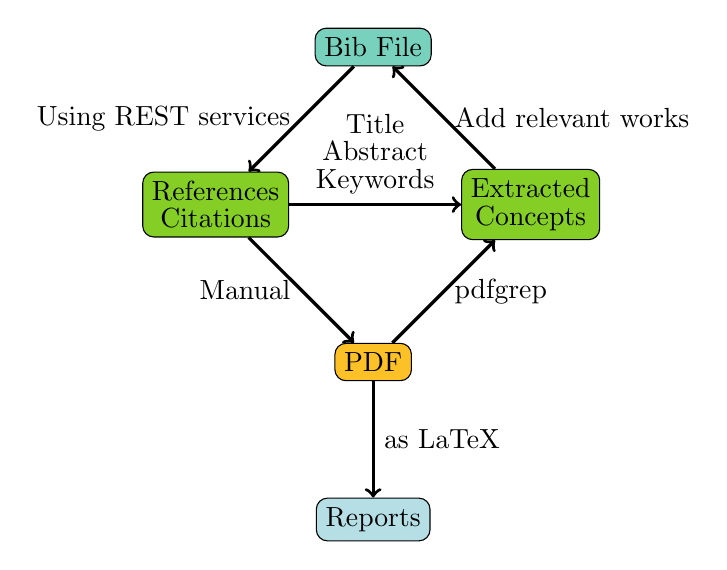
\begin{tikzpicture}[xscale=2,yscale=2]
\node[draw=black,fill=pantone_127_4,rounded corners] (bib) at (2,4) {Bib File};
\node[draw=black,fill=pantone_157_8,rounded corners] (refs) at (1,3) {\shortstack{References\\Citations}};
\node[draw=black,fill=pantone_10_7,rounded corners] (works) at (2,2) {PDF};
\node[draw=black,fill=pantone_157_8,rounded corners] (concepts) at (3,3) {\shortstack{Extracted\\Concepts}};
\node[draw=black,fill=pantone_119_1,rounded corners] (reports) at (2,1) {Reports};
\draw[very thick,black,->] (bib) -- node[left] {Using REST services} (refs);
\draw[very thick,black,->] (refs) -- node[left] {Manual} (works);
\draw[very thick,black,->] (refs) -- node[above] {\shortstack{Title\\Abstract\\Keywords}} (concepts);
\draw[very thick,black,->] (works) -- node[right] {as LaTeX} (reports);
\draw[very thick,black,->] (works) -- node[right] {pdfgrep} (concepts);
\draw[very thick,black,->] (concepts) -- node[right] {Add relevant works} (bib);
\end{tikzpicture}


\caption{\label{fig:process}Process}
\end{figure}

Our main data feed is OpenCitations~\cite{Peroni2020}, which provides both references and citing works for a given DOI key. We also use the platforms Crossref~(\url{https://www.crossref.org/documentation/}) and Scopus (\url{https://www.elsevier.com/products/scopus})
with their public REST APIs, which provide more detailed metadata for each work. 

\section{Case Studies}

So far, we have used the tool to create four surveys in different computer science areas, a summary overview is given in Table~\ref{tab:casestudies}. Each survey starts with a seed library, for example, we used a DBLP~(\url{https://dblp.org/}) search for "Constraint Programming and Scheduling" as a starting point. We use a manually defined, survey-specific ontology to find relevant papers and to find sub-categories within the survey. Existing ontologies for Computer Science~\cite{Beck2020} are not fine-grained enough for the very specialized subject areas we are interested in. Note that the number of works included in the survey is only a small fraction of all works considered. That number far exceeds the number of publications we could check manually.

\begin{table}[htbp]
\caption{\label{tab:casestudies}Survey Case Studies}
\begin{tabular}{lllrrr}\toprule
Topic & \shortstack{Work\\With} & \shortstack{Seed\\Library} & \shortstack{Ontology\\Terms} & \shortstack{Works\\Found} & \shortstack{Works\\Considered}\\ \midrule 
%CP \& Scheduling &suppressed  & \shortstack[l]{DBLP\\223}& 407 & 1,263 & 28,313\\\midrule 
%Medical \& Drones & suppressed & \shortstack[l]{WoS\\106} & 119& 495 & 14,681\\\midrule 
%AI \& Counter-Terrorism & suppressed & \shortstack[l]{Book\\32} & 183 & 1,603 & 75,792\\\midrule
%Uncertain \& CP & suppressed & \shortstack[l]{Manual\\6} & 13 & 106 & 3,328\\
CP \& Scheduling &\shortstack[l]{H. Simonis\\C. Öztürk}  & \shortstack[l]{DBLP\\223}& 407 & 1,263 & 28,313\\\midrule 
Medical \& Drones & \shortstack[l]{G. Tacadao\\B. O'Sullivan\\L. Quesada\\H. Simonis} & \shortstack[l]{WoS\\106} & 119& 495 & 14,681\\\midrule 
AI \& Counter-Terrorism & \shortstack[l]{H. Simonis\\B. O'Sullivan} & \shortstack[l]{Book\\32} & 183 & 1,603 & 75,792\\\midrule
Uncertain \& CP & \shortstack[l]{J. Lopez\\H. Simonis} & \shortstack[l]{Manual\\6} & 13 & 106 & 3,328\\
\bottomrule
\end{tabular} 
\end{table}


\subsection{Survey Example}

The current results of the "CP \& Scheduling" survey can be found online at 
%\textbf(url suppressed for review)
\url{https://hsimonis.github.io/pthg24/}, 
which also includes the sources of the application. The results are presented in different forms, based on type of publication, year of publication, the citation numbers for each work, and the number of internal connections inside the survey.

Figure~\ref{fig:mostcited} shows a list view of the most cited papers in the survey. Each line shows key properties of a work, with hyperlinks leading to more detailed information, or the paper itself. The citation numbers for each paper vary with the data feed, we use the maximum value of any feed for ranking. Note that the number of citations can be very different from the number of connections in the survey. The paper MintonJPL92\cite{MintonJPL92} in the list for example has a large number of citations, but it is not referred to by other papers in the survey. This indicates that while this is an important paper for AI in general, its influence on CP Based Scheduling is quite limited. You can also see that the estimated relevance of that paper is quite low, just above the cut-off limit.
\begin{figure}[htbp]
\includegraphics[width=\textwidth]{images/mostcited}
\caption{\label{fig:mostcited}Most Cited Works in Survey}
\end{figure}

Another type of analysis is based on the ontology, Figure~\ref{fig:concepts} shows a few of the application area concepts that we have defined, together with papers that match each concept either a lot, somewhat or only in a limited way. We see for example that \emph{farming} is not a popular concept in the survey, while \emph{maintenance scheduling} is. 
\begin{figure}[htbp]
\includegraphics[width=\textwidth]{images/concepts}
\caption{\label{fig:concepts}Works Discussing Specific Concepts}
\end{figure}

The analysis also presents an summary of each work, with key extracted information, a justification for the considered relevance score, and a list of the most similar works based on the extracted ontology features.

\subsection{Bibliometric Analysis}

We now present some of the bibliometric analysis~\cite{Donthu2021} results for the "CP \& Scheduling" survey.

Figure~\ref{fig:byinstitution} shows the institutions with the largest number of works included in the survey. The leads are the University of Toronto and the University of Bologna, but a significant number of other institutions were producing multiple works in this area. Note that this information is based on the affiliation meta-data provided in one of the data feeds, and considers the affiliation at the time of publication only. 

\begin{figure}[htbp]
\includegraphics[width=\textwidth]{images/byinstitution}
\caption{\label{fig:byinstitution}Publications by Institution}
\end{figure}

The next Figure (Figure~\ref{fig:byyear}) shows the number of publications by year, starting with early work in the 1980s. We distinguish conference papers, journal articles and PhD theses. The number of theses is probably still underrepresented, as they often miss DOI keys, and are therefore not found through database searches. It is interesting to see that since 2018 the number of journal articles outstrips the conference papers, whose numbers by year have been quite stable over time. While this may indicate a growing interest in CP based scheduling in the OR field, it can also be explained to a large part by the appearance of new actors in the scientific publishing field. Our full analysis report contains a more detailed discussion of this question.

\begin{figure}[htbp]
\includegraphics[width=\textwidth]{images/byyear}
\caption{\label{fig:byyear}Publications by Year}
\end{figure}

Figure~\ref{fig:coauthorgraph} shows a co-author graph produced from the survey data. Nodes represent authors, with the colors indicating the number of publications in the survey. Links connect authors who were coauthors for some publications, with color again indicating the number of collaborations. The graph shows that over time the CP scheduling community has worked together in many different combinations, with one large connected component of authors dominating the field, while there are only a few connected components of authors that are more isolated. This is not always the case, one of the other surveys shows that the co-author graph consists of many small connected components.  

\begin{figure}[htbp]
\centering
\includegraphics[width=10cm]{images/fdp}
%\includegraphics[width=\textwidth]{images/fdp}
\caption{\label{fig:coauthorgraph}Coauthor Graph}
\end{figure}

Finally, Figure~\ref{fig:similarity} shows the distribution of the cosine similarity measure based on the ontology features that we extract from the full text version of the works. We see that there are a few papers that are considered to be very similar to each other, these typically are papers by the same authors in different settings, for example a conference paper followed by an extended journal version of that paper. The similarity values are used in the survey to identify the closest works related to some specific paper, which might be of interest to readers of selected papers.

\begin{figure}[htbp]
\centering
\includegraphics[width=12cm]{images/similaritydistributioncosine}
\caption{\label{fig:similarity}Similarity Distribution}
\end{figure}

\section{Limitations and Future Work}

While the tool already has shown its usefulness in generating surveys of specific Computer Science areas, we have identified several limitations that we may resolve in future versions.

The primary limitation arises from the fact that none of the database providers offer comprehensive data, which restricts the scope of the analyses we can conduct. For example, the abstract of a work is not always available in the meta-data, limiting our relevance analysis without access to the full text. As the database queries are using the DOI keys to identify works, they are not very helpful in analyzing works that do not have a DOI. This is a problem in particular for PhD theses, where universities have not assigned a DOI, and for older (before 2005) AI conferences, which were published by AI societies. For the "CP \& Scheduling" survey we did perform a manual search of the proceedings by hand to find all relevant early publications on the topic. Finally, the use of one specific ontology in English for an area may result in ignoring works published in other languages that will use other technical terms for the same concepts. The use of a LaTeX tool-chain and non-uniform encoding of characters in web searches causes issues for non-Latin texts. We did find that while retrieving the full-text versions remains a manual process, this was not a limiting factor, as we could present the required links and keys to the user in a way that allowed very rapid access (less than a minute per paper). 

There are of course further analysis that can be performed on the collected papers, for example visualizing the connection between all papers for a specific sub-area, to see when novel concepts were first introduced. This could help with providing further analysis of the publications in an area for a deeper understanding of a sub-field.   


\begin{acknowledgments}
%suppressed for review
This publication has emanated from research conducted with the financial support of Science Foundation Ireland under Grant number  12/RC/2289-P2 at Insight the SFI Research Centre for Data %Analytics at UCC, which is co-funded under the European Regional Development Fund. For the purpose of Open Access, the author has applied a CC BY public copyright licence to any Author %Accepted Manuscript version arising from this submission. 
\end{acknowledgments}

%%
%% Define the bibliography file to be used
\bibliography{bib}


\end{document}

%%
%% End of file
